\documentclass{article}
\usepackage[utf8]{inputenc}
\usepackage{listings}
\usepackage{graphicx}
\usepackage{float}
\usepackage{xcolor}
\usepackage{geometry}
\usepackage{CJKutf8}
\usepackage{amsmath}
\usepackage{amssymb}

\geometry{a4paper,scale=0.8}
\lstset{
    basicstyle          =   \sffamily,        
    keywordstyle        =   \bfseries,         
    commentstyle        =   \rmfamily\itshape, 
    stringstyle         =   \ttfamily, 
    flexiblecolumns,               
    numbers             =   left,  
    showspaces          =   false, 
    showstringspaces    =   false,
    captionpos          =   t,     
    frame               =   lrtb, 
}

\lstdefinestyle{Python}{
    language        =   Python, % 语言选Python
    basicstyle      =   \zihao{-5}\ttfamily,
    numberstyle     =   \zihao{-5}\ttfamily,
    keywordstyle    =   \color{blue},
    keywordstyle    =   [2] \color{teal},
    stringstyle     =   \color{magenta},
    commentstyle    =   \color{red}\ttfamily,
    breaklines      =   true,  
    columns         =   fixed,  
    basewidth       =   0.5em,
}

\title{\bf\Large  概率论与数理统计 第5次作业}
%%%%%%%%%%%%%%%%%%%%%%%%%%%%%%%%%%%%%%
%% DON'T forget to change this part %%
\author{\bf Name: 宋昊原 \qquad Student ID: 2022010755}
%%%%%%%%%%%%%%%%%%%%%%%%%%%%%%%%%%%%%%

\begin{document}
\begin{CJK}{UTF8}{gbsn}
\maketitle
\section{取球}
\subsection{}
$$ P(X=x,Y=y)=\frac{3!}{x!y!(3-x-y)!}(\frac{3}{12})^{x}(\frac{4}{12})^{y}(\frac{5}{12})^{3-x-y}$$
于是\\
\begin{tabular}{c|c|c|c|c}
	(X,Y) & (0,Y) & (1,Y) & (2,Y) & (3,Y)\\
	\hline
	(X,0) & $\frac{125}{1728}$ & $\frac{225}{1728}$ & $\frac{135}{1728}$ & $\frac{27}{1728}$\\
    \hline
    (X,1) & $\frac{300}{1728}$ & $\frac{360}{1728}$ & $\frac{108}{1728}$ & $0$\\
    \hline
    (X,2) & $\frac{240}{1728}$ & $\frac{144}{1728}$ & $0$ & $0$\\
    \hline
    (X,3) & $\frac{64}{1728}$ & $0$ & $0$ & $0$\\
    \hline
\end{tabular}
\subsection{}
$$ P(X=1)=\sum\limits_{j=0}^{3}P(X=1,Y=j)=\frac{729}{1728}=\frac{27}{64}$$
\section{联合分布的公式}
$$ F(b,d)-F(a,d)-F(b,c)+F(a,c)=(F(b,d)-F(a,d))-(F(b,c)-F(a,c))$$
$$ =(P(X\leq b,Y\leq d)-P(X\leq a,Y\leq d))-(P(X\leq b,Y\leq c)-P(X\leq a,Y\leq c))$$
$$ =P(a<X\leq b,Y\leq d)-P(a<X\leq b,Y\leq c)$$
$$ =P(a<X\leq b,c<Y\leq d)$$
\section{圆盘均匀分布}
\subsection{}
\begin{equation}
    f(x,y)=\left\{
    \begin{array}{cl}
    \frac{1}{\pi} & x^{2}+y^{2}\leq 1\\
    0 & else\\
    \end{array}\right.
\end{equation}
\subsection{}
$$ f_{X}(x)=\int_{-\infty}^{+\infty}f(x,y)dy=\int_{-\sqrt{1-x^{2}}}^{\sqrt{1-x^{2}}}\frac{1}{\pi}dy=2\frac{\sqrt{1-x^{2}}}{\pi}$$
同理
$$ f_{Y}(y)=2\frac{\sqrt{1-y^{2}}}{\pi} $$
\subsection{}
$$P(R\leq r)=\iint_{x^{2}+y^{2}\leq r^{2}}f(x,y)dxdy=\frac{\pi r^{2}}{\pi}=r^{2}$$
\subsection{}
将R视为一个新的随机变量,则其概率密度函数
$$f_{R}(r)=\frac{d}{dr}P(R\leq r)=2r,\forall r\in [0,1]$$
则
$$ E(R)=\int_{0}^{1}rf_{R}(r)dr=\int_{0}^{1}2r^{2}dr=\frac{2}{3}$$
\section{二元正态分布的边际密度}
首先给出二元正态分布的PDF
$$ f(x,y)=\frac{1}{2\pi\sigma_{1}\sigma_{2}\sqrt{1-\rho^{2}}}\exp{(-\frac{1}{2(1-\rho^{2})}((\frac{x-\mu_{1}}{\sigma_{1}})^{2}+(\frac{y-\mu_{2}}{\sigma_{2}})^{2}-2\rho\frac{(x-\mu_{1})(y-\mu_{2})}{\sigma_{1}\sigma_{2}}))}$$
其对X的边际密度为
$$ f_{X}(x)=\int_{-\infty}^{+\infty}f(x,y)dy$$
令$\xi=\frac{x-\mu_{1}}{\sigma_{1}}$,$\eta=\frac{y-\mu_{2}}{\sigma_{2}}$,则
$$ f_{X}(x)=\frac{1}{2\pi\sigma_{1}\sigma_{2}\sqrt{1-\rho^{2}}}\int_{-\infty}^{+\infty}\exp{(-\frac{1}{2(1-\rho^{2})}(\xi^{2}+\eta^{2}-2\rho\xi\eta))}d(\sigma_{2}\eta+\mu_{2})$$
$$ =\frac{1}{2\pi\sigma_{1}\sqrt{1-\rho^{2}}}\int_{-\infty}^{+\infty}\exp{(-\frac{1}{2(1-\rho^{2})}((\eta-\rho\xi)^{2}+(1-\rho^{2})\xi^{2}))}d\eta$$
$$ =\frac{1}{2\pi\sigma_{1}\sqrt{1-\rho^{2}}}\exp(-\frac{1}{2}\xi^{2})\int_{-\infty}^{+\infty}\exp{(-\frac{1}{2(1-\rho^{2})}(\eta-\rho\xi)^{2})}d\eta$$
$$ =\frac{1}{2\pi\sigma_{1}\sqrt{1-\rho^{2}}}\exp(-\frac{1}{2}\xi^{2})\int_{-\infty}^{+\infty}\exp{(-(\frac{\eta-\rho\xi}{\sqrt{2(1-\rho^{2})}})^{2})}d\eta$$
$$ =\frac{1}{\sqrt{2}\pi\sigma_{1}}\exp(-\frac{1}{2}\xi^{2})\int_{-\infty}^{+\infty}\exp{(-(\frac{\eta-\rho\xi}{\sqrt{2(1-\rho^{2})}})^{2})}d\frac{\eta-\rho\xi}{\sqrt{2(1-\rho^{2})}}$$
$$ =\frac{1}{\sqrt{2}\pi\sigma_{1}}\exp(-\frac{1}{2}\xi^{2})\int_{-\infty}^{+\infty}\exp{(-(\frac{\eta-\rho\xi}{\sqrt{2(1-\rho^{2})}})^{2})}d\frac{\eta-\rho\xi}{\sqrt{2(1-\rho^{2})}}$$
$$ =\frac{1}{\sqrt{2\pi}\sigma_{1}}e^{-\frac{\xi^{2}}{2}}$$
$$ =\frac{1}{\sqrt{2\pi}\sigma_{1}}e^{-\frac{(x-\mu_{1})^{2}}{2\sigma_{1}^{2}}}$$
相当于一元正态分布.
\\同理
$$ f_{Y}(y)=\frac{1}{\sqrt{2\pi}\sigma_{2}}e^{-\frac{(y-\mu_2)^{2}}{2\sigma_{2}^{2}}}$$
\section{二元正态分布的条件密度}
$$ f_{X|Y}(x|y)=\frac{f(x,y)}{f_{Y}(y)}$$
$$ =\frac{\frac{1}{2\pi\sigma_{1}\sigma_{2}\sqrt{1-\rho^{2}}}\exp{(-\frac{1}{2(1-\rho^{2})}((\frac{x-\mu_{1}}{\sigma_{1}})^{2}+(\frac{y-\mu_{2}}{\sigma_{2}})^{2}-2\rho\frac{(x-\mu_{1})(y-\mu_{2})}{\sigma_{1}\sigma_{2}}))}}{\frac{1}{\sqrt{2\pi}\sigma_{2}}e^{-\frac{(y-\mu_{2})^{2}}{2\sigma_{2}^{2}}}}$$
$$ =\frac{1}{\sqrt{2\pi(1-\rho^{2})}\sigma_{1}}\exp{(-\frac{1}{2(1-\rho^{2})}((\frac{x-\mu_{1}}{\sigma_{1}})^{2}+(\rho\frac{y-\mu_{2}}{\sigma_{2}})^{2}-2\rho\frac{(x-\mu_{1})(y-\mu_{2})}{\sigma_{1}\sigma_{2}}))}$$
$$ =\frac{1}{\sqrt{2\pi(1-\rho^{2})}\sigma_{1}}\exp{(-\frac{1}{2(1-\rho^{2})}(\frac{x-\mu_{1}}{\sigma_{1}}-\rho\frac{y-\mu_{2}}{\sigma_{2}})^{2})}$$
\section{三角形域内的均匀分布}
\subsection{联合分布}
设三角形域为D,则
\begin{equation}
    f(x,y)=\left\{
    \begin{array}{cl}
    2 & (x,y)\in D\\
    0 & else\\
    \end{array}\right.
\end{equation}
\subsection{边际分布}
$$ f_{Y}(y)=\int_{-\infty}^{+\infty}f(x,y)dx$$
$$ =\int_{0}^{1-y}2dx$$
$$ =1-y,\forall y\in [0,1]$$
\subsection{条件分布}
$$ f_{X|Y}(x|y)=\frac{f(x,y)}{f_{Y}(y)}$$
$$ =\frac{2}{1-y},\forall (x,y)\in D$$
\section{独立随机变量}
\subsection{条件分布}
条件分布的PMF:
$$ f_{X_{1}|X_{1}+X_{2}}(m|n)=\frac{f_{X_{1},X_{2}}(m,n-m)}{f_{X_{1}+X_{2}}(n)}$$
$$ =\frac{f_{X_{1}}(m)f_{X_{2}}(n-m)}{f_{X_{1}+X_{2}}(n)}$$
$$ =\frac{\frac{\lambda_{1}^{m}}{m!}e^{-\lambda_{1}}\frac{\lambda_{2}^{n-m}}{(n-m)!}e^{-\lambda_{2}}}{\frac{(\lambda_{1}+\lambda_{2})^{n}}{n!}e^{-\lambda_{1}-\lambda_{2}}}$$
$$ =\tbinom{n}{m}(\frac{\lambda_{1}}{\lambda_{1}+\lambda_{2}})^{m}(\frac{\lambda_{2}}{\lambda_{1}+\lambda_{2}})^{n-m}$$
\subsection{解释}
上述条件分布质量函数在形式上接近二项分布. 事实上,这种情形在语义上也接近二项分布.
\\这里$X_{1}$和$X_{2}$服从泊松分布的含义可以认为是:对一个系统观测一段时间,其中事件1发生的次数为$X_{1}$,事件2发生的次数为$X_{2}$.
\\当前语境下,已知事件1和2共发生了n次,求此条件下事件1发生m次的概率,这非常类似于二项分布.
\\同时,由于$\lambda_{1}$和$\lambda_{2}$分别为这段时间内发生事件1和2的次数的期望值,因此可以认为从发生的每个事件中随机抽一个事件,是事件1、事件2的概率的比值为$\frac{\lambda_{1}}{\lambda_{2}}$.
\\也就是,这个条件分布其实是$B(n,\frac{\lambda_{1}}{\lambda_{1}+\lambda_{2}})$.
\section{约定见面}
规定两人到达时间以2点为1,1点为0,均匀分划刻度.
\subsection{}
\begin{equation}
    f(x,y)=\left\{
    \begin{array}{cl}
    1 & (x,y)\in D=[0,1]\times[0,1]\\
    0 & else\\
    \end{array}\right.
\end{equation}
\subsection{}
这里要求的事件相当于以下条件:
$$ X-Y>\frac{1}{6}\lor Y-X>\frac{1}{6}$$
D是单位正方形,而D中的上述区域(设为A)相当于2个直角边长为$\frac{5}{6}$的等腰直角三角形. 则
$$ P((x,y)\in A)=\int_{A}f(x,y)dxdy=\int_{A}dxdy=S(A)=\frac{25}{36}$$
即所求概率为$\frac{25}{36}$.
\section{Farlie-Morgenstein族}
\subsection{}
$$ H_{X}(x)=\lim\limits_{y\to+\infty}H(x,y)$$
$$ =\lim\limits_{y\to+\infty}F(x)G(y)\{1+\alpha[1-F(x)][1-G(y)]\}$$
由于
$$\lim\limits_{y\to+\infty}G(y)=1$$
有
$$ H_{X}(x)=F(x)$$
同理
$$ H_{Y}(y)=G(y)$$
\subsection{}
这里只需要讨论$(x,y)\in D=[0,1]\times[0,1]$的情况.
\\此时,$F(x)=x,G(y)=y$.
\\对于$\alpha=1$,有
$$ H_{1}(x,y)=xy(1-(1-x)(1-y))=x^{2}y+xy^{2}-x^{2}y^{2}$$
求出$D$上的概率密度函数($D$外恒取0)
$$ h_{1}(x,y)=\frac{\partial^{2}}{\partial x\partial y}H_{1}(x,y)=2x+2y-4xy$$
同理,对于$\alpha=-1$
$$ H_{2}(x,y)=2xy-x^{2}y-xy^{2}+x^{2}y^{2}$$
$$ h_{2}(x,y)=2-2x-2y+4xy$$
\section{Copula函数}
令
$$ H(x,y)=C(F(x),G(y))$$
由于$C(u,v)$是连续分布的联合累积分布,它在$\mathbb{R}^{2}$内任何一点都应当连续.
于是
$$ H_{X}(x)=\lim\limits_{y\to+\infty}H(x,y)=C(F(x),G(+\infty))=C(F(x),1)$$
由于$C(u,v)$对X和Y的边际分布都是$[0,1]$上均匀分布
$$ C(F(x),1)=C_{X}(F(x))=F(x) $$
于是
$$ H_{X}(x)=F(x)$$
同理
$$ H_{Y}(y)=G(y)$$
\section{全概率公式和Bayes公式}
在接下来的讨论中,我们都研究$f_{X}(x)$的全概率公式和$f_{Y|X}(y|x)$的Bayes公式,也就是在$X=x$发生的情况下推断$Y=y$发生的后验概率.
\\将指出,这一公式的形式与X是连续还是离散无关,只与Y有关,但这只是形式上的. 实际上相应的函数$f$要根据X是离散还是连续选择理解成PMF还是PDF.
\subsection{Y离散的情形}
全概率公式
$$ f_{X}(x)=\sum\limits_{y}f_{X|Y}(x|y)f_{Y}(y) $$
Bayes公式
$$ f_{Y|X}(y_{0}|x)=\frac{f_{X|Y}(x|y_{0})f_{Y}(y_{0})}{\sum\limits_{y}f_{X|Y}(x|y)f_{Y}(y)}$$
\subsection{Y连续的情形}
全概率公式
$$ f_{X}(x)=\int_{-\infty}^{+\infty}f_{X|Y}(x|y)f_{Y}(y)dy $$
Bayes公式
$$ f_{Y|X}{y_{0}|x}=\frac{f_{X|Y}(x|y_{0})f_{Y}(y_{0})}{\int_{-\infty}^{+\infty}f_{X|Y}(x|y)f_{Y}(y)dy}$$
\section{}
\subsection{}
由$f(x,y)$是PDF,应有
$$ \iint\limits_{x^{2}+y^{2}\leq 1}\frac{c}{1+x^{2}+y^{2}}dxdy = 1$$
作极坐标变换,有
$$ \int_{0}^{2\pi}(\int_{0}^{1}\frac{c\rho}{1+\rho^{2}}d\rho)d\phi $$
$$ =\pi\int_{0}^{1}\frac{c}{1+\rho^{2}}d(1+\rho^{2})$$
$$ =\pi c\ln(1+\rho^{2})|_{0}^{1}$$
$$ =\pi c\ln 2=1 $$
于是
$$ c=\frac{1}{\pi\ln2}$$
\subsection{}
$$ f_{X}(x)=\int_{-\infty}^{+\infty}f(x,y)dy $$
$$ =\int_{-\sqrt{1-x^{2}}}^{\sqrt{1-x^{2}}}\frac{1}{\pi\ln2(1+x^{2}+y^{2})}dy$$
$$ =\frac{1}{\pi\ln2\sqrt{1+x^{2}}}\int_{-\sqrt{1-x^{2}}}^{\sqrt{1-x^{2}}}\frac{1}{(\frac{y}{\sqrt{1+x^{2}}})^{2}+1}d\frac{y}{\sqrt{1+x^{2}}}$$
$$ =\frac{1}{\pi\ln2\sqrt{1+x^{2}}}\arctan\frac{y}{\sqrt{1+x^{2}}}|_{-\sqrt{1-x^{2}}}^{\sqrt{1-x^{2}}}$$
$$ =\frac{2}{\pi\ln2\sqrt{1+x^{2}}}\arctan{\sqrt{\frac{1-x^{2}}{1+x^{2}}}}$$
同理
$$ f_{Y}(y)=\frac{2}{\pi\ln2\sqrt{1+y^{2}}}\arctan{\sqrt{\frac{1-y^{2}}{1+y^{2}}}}$$
考虑$(0,0)$点
$$ f_{X}(0)=f_{Y}(0)=\frac{1}{2\ln2}$$
$$ f(0,0)=c=\frac{1}{\pi\ln2}$$
故
$$ f(0,0)\neq f_{X}(0)f_{Y}(0) $$
于是X和Y不独立.
\section{边际正态分布但不是二元正态分布的反例}
\subsection{}
只需证明$g(x,y)\geq 0$且$\iint\limits_{\mathbb{R}^{2}}g(x,y)dxdy=1$.
\\由于$X,Y\sim N(0,1)$且X和Y独立
$$ f(x,y)=\frac{1}{2\pi}\exp{(-\frac{x^{2}+y^{2}}{2})}$$
$\forall (x,y)\in D=\{(x,y)|x^{2}+y^{2}\leq 1\}$,有
$$ \frac{e^{-\frac{1}{2}}}{2\pi}\leq f(x,y)\leq \frac{1}{2\pi}$$
而
$$ |\frac{xy}{100}|\leq \frac{1}{200}<\frac{e^{-\frac{1}{2}}}{2\pi}$$
故在D上
$$ g(x,y)=f(x,y)+\frac{xy}{100}\geq 0$$
而在D外$g(x,y)=f(x,y)$非负,这证明了非负性.
\\要证明归一性,只需要证明在D上$g$和$f$积分相同,即
$$ \iint\limits_{D}\frac{xy}{100}dxdy=0$$
由于$\frac{xy}{100}$关于$x$轴对称,这个积分确实为0,这证明了归一性.
\\于是$g(x,y)$是一个二维概率密度函数.
\subsection{}
考虑$U$的边际分布
$$ g_{U}(x)=\int_{-\infty}^{+\infty}g(x,y)dy$$
$$ =\int_{-\infty}^{+\infty}f(x,y)dy+\phi(x)$$
上述第一项就是标准正态分布,考虑余项$\phi(x)$,当$x\notin (-1,1)$时,$\phi(x)=0$,只需考虑$x\in(-1,1)$的情形,此时
$$ \phi(x)=\int_{-\sqrt{1-x^{2}}}^{\sqrt{1-x^{2}}}\frac{xy}{100}dy$$
这是奇函数在对称区间上的积分,为0. 于是$U\sim N(0,1)$,同理,$V\sim N(0,1)$.
\\然而,二元正态分布的概率密度函数是连续函数,而$g(x,y)$在任何满足
$$ x^{2}+y^{2}=1\land xy\neq 0$$
的点不连续,因此$(U,V)$不服从二元正态分布.
\section{计算机实验:随机变量的函数}
以下是$x_{i}$的直方图与指数分布概率密度函数的比较,其中红色曲线为指数分布概率密度函数.
\\
\begin{minipage}{0.5\textwidth}
    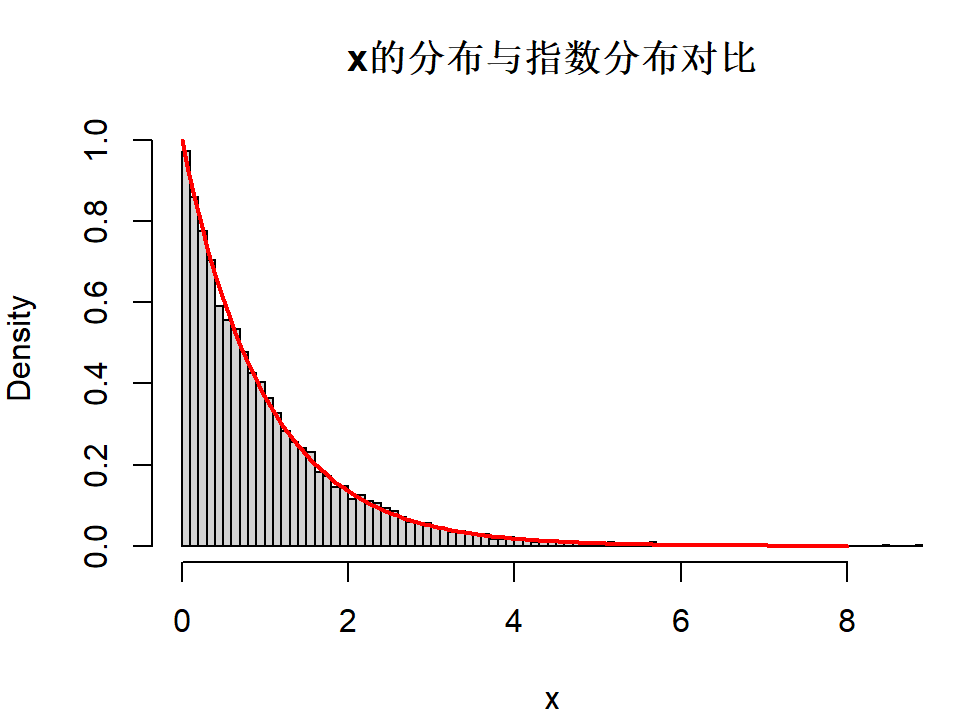
\includegraphics[scale=0.6]{plot.png}
\end{minipage}
\\
以下是我使用的代码.
\\
\begin{minipage}{0.5\textwidth}
    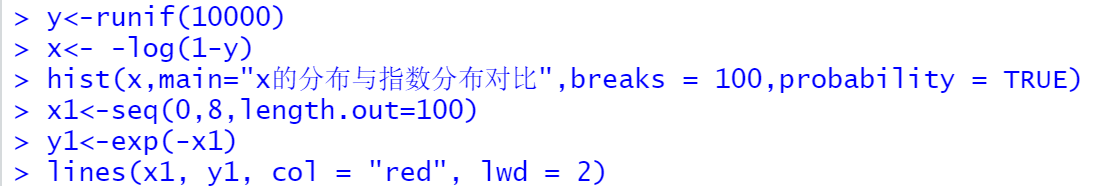
\includegraphics[scale=0.6]{code.png}
\end{minipage}
\end{CJK}
\end{document}